\chapter{Graphs and plots}
\label{chap-graphs}



\section{Gnuplot graphs}
\label{gnuplot-graphs}



\subsection{General gnuplot options}
\label{gnuplot-opts}

A separate program, \app{gnuplot}, is called to generate graphs.
Gnuplot is a very full-featured graphing program with myriad options.
It is available from \href{http://www.gnuplot.info/}{www.gnuplot.info}
(but note that a copy of gnuplot is bundled with the MS Windows
version of \app{gretl}).  \app{gretl} gives you direct access, via a
graphical interface, to a subset of gnuplot's options and it tries to
choose sensible values for you; it also allows you to take complete
control over graph details if you wish.With a graph displayed, you can
click on the graph window for a pop-up menu with the following
options.

\begin{itemize}
\item \textsf{Save as PNG}: Save the graph in Portable Network
  Graphics format.
\item \textsf{Save as postscript}: Save in encapsulated postscript
  (EPS) format.
\item \textsf{Save as Windows metafile}: Save in Enhanced Metafile
  (EMF) format.
\item \textsf{Save to session as icon}: The graph will appear in
  iconic form when you select "Icon view" from the Session menu.
\item \textsf{Zoom}: Lets you select an area within the graph for
  closer inspection (not available for all graphs).
\item \textsf{Print}: On the Gnome desktop only, lets you print the
  graph directly.
\item \textsf{Copy to clipboard}: MS Windows only, lets you paste the
  graph into Windows applications such as MS Word.\footnote{For best
    results when pasting graphs into MS Office applications, choose
    the application's ``Edit, Paste Special...'' menu item, and select
    the option ``Picture (Enhanced Metafile)''.}
\item \textsf{Edit}: Opens a controller for the plot which lets you
  adjust various aspects of its appearance.
\item \textsf{Close}: Closes the graph window.
\end{itemize}


\subsection{Displaying data labels}
\label{plot-labels}

In the case of a simple X-Y scatterplot (with or without a line of
best fit displayed), some further options are available if the dataset
includes ``case markers'' (that is, labels identifying each
observation).\footnote{For an example of such a dataset, see the
  Ramanathan file \verb+data4-10+: this contains data on private
  school enrollment for the 50 states of the USA plus Washington, DC;
  the case markers are the two-letter codes for the states.} With a
scatter plot displayed, when you move the mouse pointer over a data
point its label is shown on the graph.  By default these labels are
transient: they do not appear in the printed or copied version of the
graph.  They can be removed by selecting ``Clear data labels'' from
the graph pop-up menu. If you want the labels to be affixed
permanently (so they will show up when the graph is printed or
copied), you have two options.
    
\begin{itemize}
\item To affix the labels currently shown on the graph, select
  ``Freeze data labels'' from the graph pop-up menu.
\item To affix labels for all points in the graph, select ``Edit''
  from the graph pop-up and check the box titled ``Show all data
  labels''.  This option is available only if there are less than 55
  data points, and it is unlikely to produce good results if the
  points are tightly clustered since the labels will tend to overlap.
\end{itemize}


To remove labels that have been affixed in either of these ways,
select ``Edit'' from the graph pop-up and uncheck ``Show all data
labels''.
    

\subsection{Advanced options}
\label{plot-advanced}

If you know something about \app{gnuplot} and wish to get finer
control over the appearance of a graph than is available via the
graphical controller (``Edit'' option), you have two further options.

\begin{itemize}
\item Once the graph is saved as a session icon, you can right-click
  on its icon for a further pop-up menu.  One of the otions here is
  ``Edit plot commands'', which opens an editing window with the
  actual gnuplot commands displayed. You can edit these commands and
  either save them for future processing or send them to gnuplot (with
  the ``File/Send to gnuplot'' menu item in the plot commands editing
  window).
\item Another way to save the plot commands (or to save the displayed
  plot in formats other than EPS or PNG) is to use ``Edit'' item on a
  graph's pop-up menu to invoke the graphical controller, then click
  on the ``Output to file'' tab in the controller.  You are then
  presented with a drop-down menu of formats in which to save the
  graph.
\end{itemize}

To find out more about \app{gnuplot} see the
\href{http://ricardo.ecn.wfu.edu/gnuplot.html}{online manual} or
\href{http://www.gnuplot.info/}{www.gnuplot.info}.See also the entry
for \cmd{gnuplot} in the \emph{Gretl Command Reference} --- and the
\cmd{graph} and \cmd{plot} commands for ``quick and dirty'' ASCII
graphs.

\begin{figure}[htbp]
  \caption{gretl's gnuplot controller}
  \label{fig-plot}
  \begin{center}
    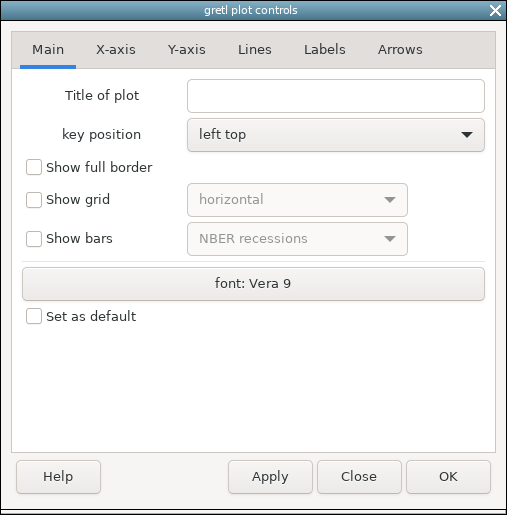
\includegraphics[scale=0.5]{figures/plot_control}
  \end{center}
\end{figure}


\section{Boxplots}
\label{sect-boxplots}

Boxplots are not generated using gnuplot, but rather by \app{gretl}
itself.These plots (after Tukey and Chambers) display the distribution
of a variable. The central box encloses the middle 50 percent of the
data, i.e. it is bounded by the first and third quartiles.  The
``whiskers'' extend to the minimum and maximum values.  A line is
drawn across the box at the median.In the case of notched boxes, the
notch shows the limits of an approximate 90 percent confidence
interval.  This is obtained by the bootstrap method, which can take a
while if the data series is very long.Clicking the mouse in the
boxplots window brings up a menu which enables you to save the plots
as encapsulated postscript (EPS) or as a full-page postscript file.
Under the X window system you can also save the window as an XPM file;
under MS Windows you can copy it to the clipboard as a bitmap.  The
menu also gives you the option of opening a summary window which
displays five-number summaries (minimum, first quartile, median, third
quartile, maximum), plus a confidence interval for the median if the
``notched'' option was chosen.  Some details of gretl's boxplots can
be controlled via a (plain text) file named \verb+.boxplotrc+ which is
looked for, in turn, in the current working directory, the user's home
directory (corresponding to the environment variable HOME) and the
gretl user directory (which is displayed and may be changed under the
``File, Preferences, General'' menu).  Options that can be set in this
way are the font to use when producing postscript output (must be a
valid generic postscript font name; the default is Helvetica), the
size of the font in points (also for postscript output; default is
12), the minimum and maximum for the y-axis range, the width and
height of the plot in pixels (default, 560 x 448), whether numerical
values should be printed for the quartiles and median (default, don't
print them), and whether outliers (points lying beyond 1.5 times the
interquartile range from the central box) should be indicated
separately (default, no).  Here is an example:

\begin{code}
font = Times-Roman
fontsize = 16
max = 4.0
min = 0
width = 400
height = 448
numbers = %3.2f
outliers = true
\end{code}

On the second to last line, the value associated with \verb+numbers+
is a ``printf'' format string as in the C programming language; if
specified, this controls the printing of the median and quartiles next
to the boxplot, if no \verb+numbers+ entry is given these values are
not printed.  In the example, the values will be printed to a width of
3 digits, with 2 digits of precision following the decimal point.Not
all of the options need be specified, and the order doesn't matter.
Lines not matching the pattern ``key = value'' are ignored, as are
lines that begin with the hash mark, \verb+#+.After each variable
specified in the boxplot command, a parenthesized boolean expression
may be added, to limit the sample for the variable in question.  A
space must be inserted between the variable name or number and the
expression.  Suppose you have salary figures for men and women, and
you have a dummy variable \verb+GENDER+ with value 1 for men and 0 for
women.  In that case you could draw comparative boxplots with the
following line in the boxplots dialog:

\begin{code}
      salary (GENDER=1) salary (GENDER=0)
\end{code}

%%% Local Variables: 
%%% mode: latex
%%% TeX-master: "gretl-guide"
%%% End: 

